\begin{frame}{Layer Normalization vs RMSNorm}
  \small
  \textbf{LayerNorm:} Normalizes across the feature dimension by subtracting the mean and dividing by the standard deviation.

  \vspace{0.5em}
  \textbf{RMSNorm:} Removes the mean and scales by the root mean square (RMS) of the features.

  \vspace{1em}
  \begin{itemize}
      \item[$\blacktriangleright$] Simpler
      \item[$\blacktriangleright$] Faster
      \item[$\blacktriangleright$] Slightly better in large-scale settings \textbf{zhou2022rmsnorm}
  \end{itemize}
\end{frame}

\begin{frame}{Layer Normalization vs RMSNorm}
  \centering
  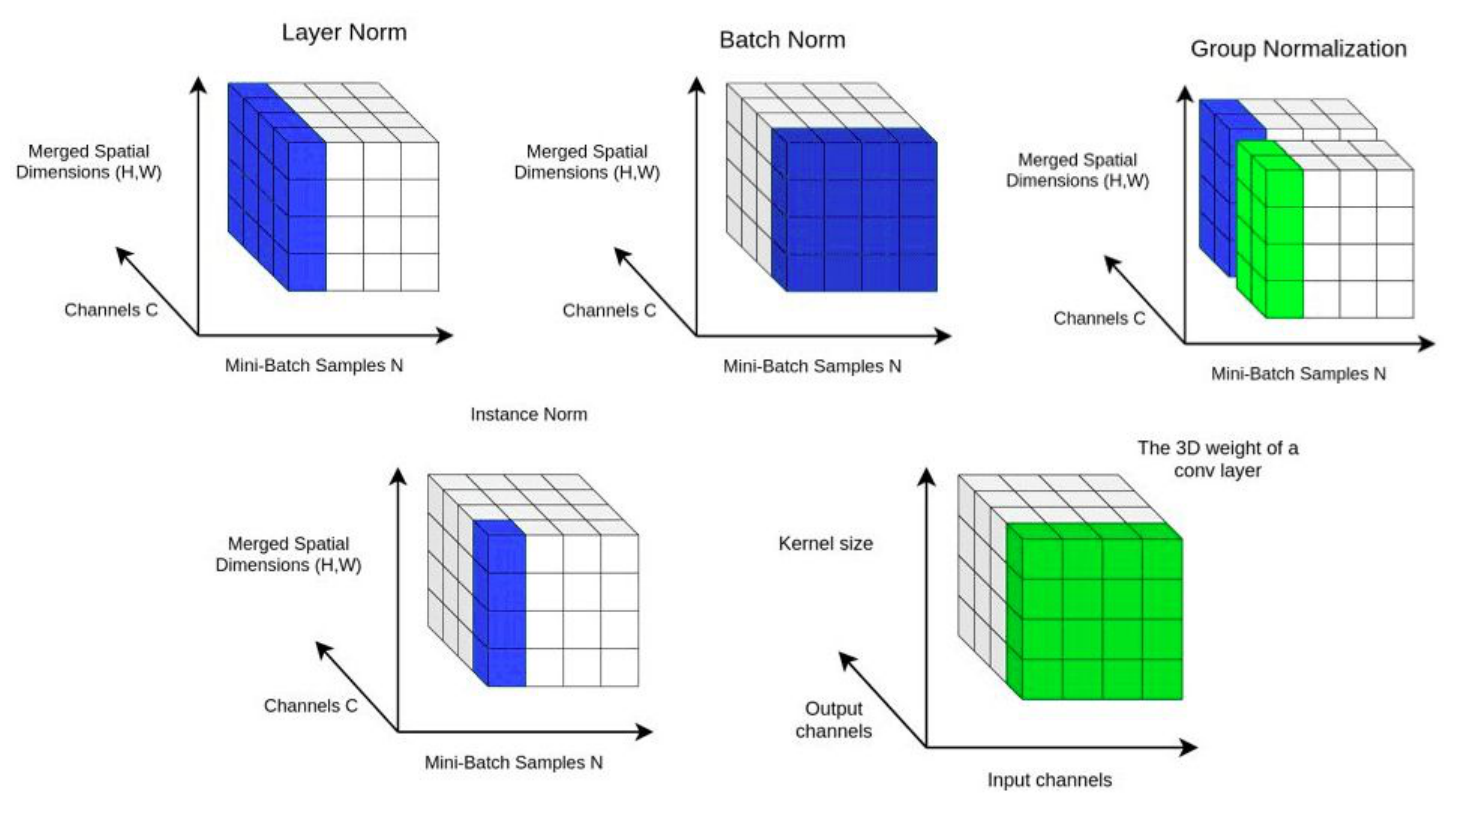
\includegraphics[width=0.8\paperwidth,height=0.8\paperheight,keepaspectratio]{assets/Lecture-6_Introduction_to_Transformers/pdf_page_088.png}
\end{frame}

\begin{frame}{Layer Normalization vs RMSNorm}
  \centering
  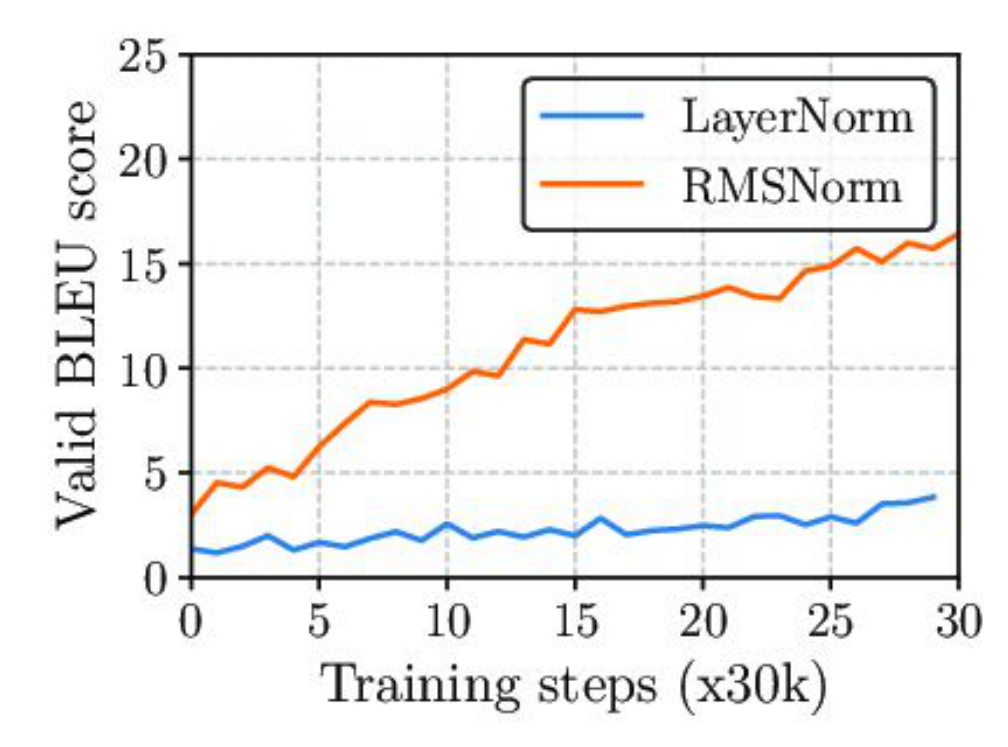
\includegraphics[width=0.8\paperwidth,height=0.8\paperheight,keepaspectratio]{assets/Lecture-6_Introduction_to_Transformers/pdf_page_089.png}
\end{frame}

